%\documentclass[12pt]{article}
%\usepackage[utf8]{inputenc}
%\usepackage[czech]{babel}
%\usepackage{a4wide}
%\usepackage{amsmath}
%\usepackage{amssymb}
%\usepackage{amsfonts}
%\begin{document}
%\section{ISS}
\chapter{Mezinárodní kosmická stanice}
Mezinárodní kosmická stanice (ISS, International Space Station) je umělá družice Země. Obíhá Zemi na orbitě se sklonem dráhy 51$^{\circ}$~\cite{ISS_wiki} v nadmořské výšce oscilující kolem 400 km rychlostí 28 800 km/h, což znamená, že celou Zem obletí každých 90 min~\cite{ISS_where}. Konstrukce stanice započala v roce 1998, od listopadu 2000 je permanentně obývána lidmi. Od roku 2009 je posádka šestičlenná, přičemž po šesti měsících se obměňují zpravidla dva její členové~\cite{ISS_wiki}. Při konstrukci stanice byly značně využívány americké raketoplány Space Shuttle, které se po dokončení stanice v roce 2011 přestaly používat. V současnosti je zásobování stanice obstaráváno ruskými kosmickými loděmi Soyuz.
\begin{figure}[H]
  \centering
  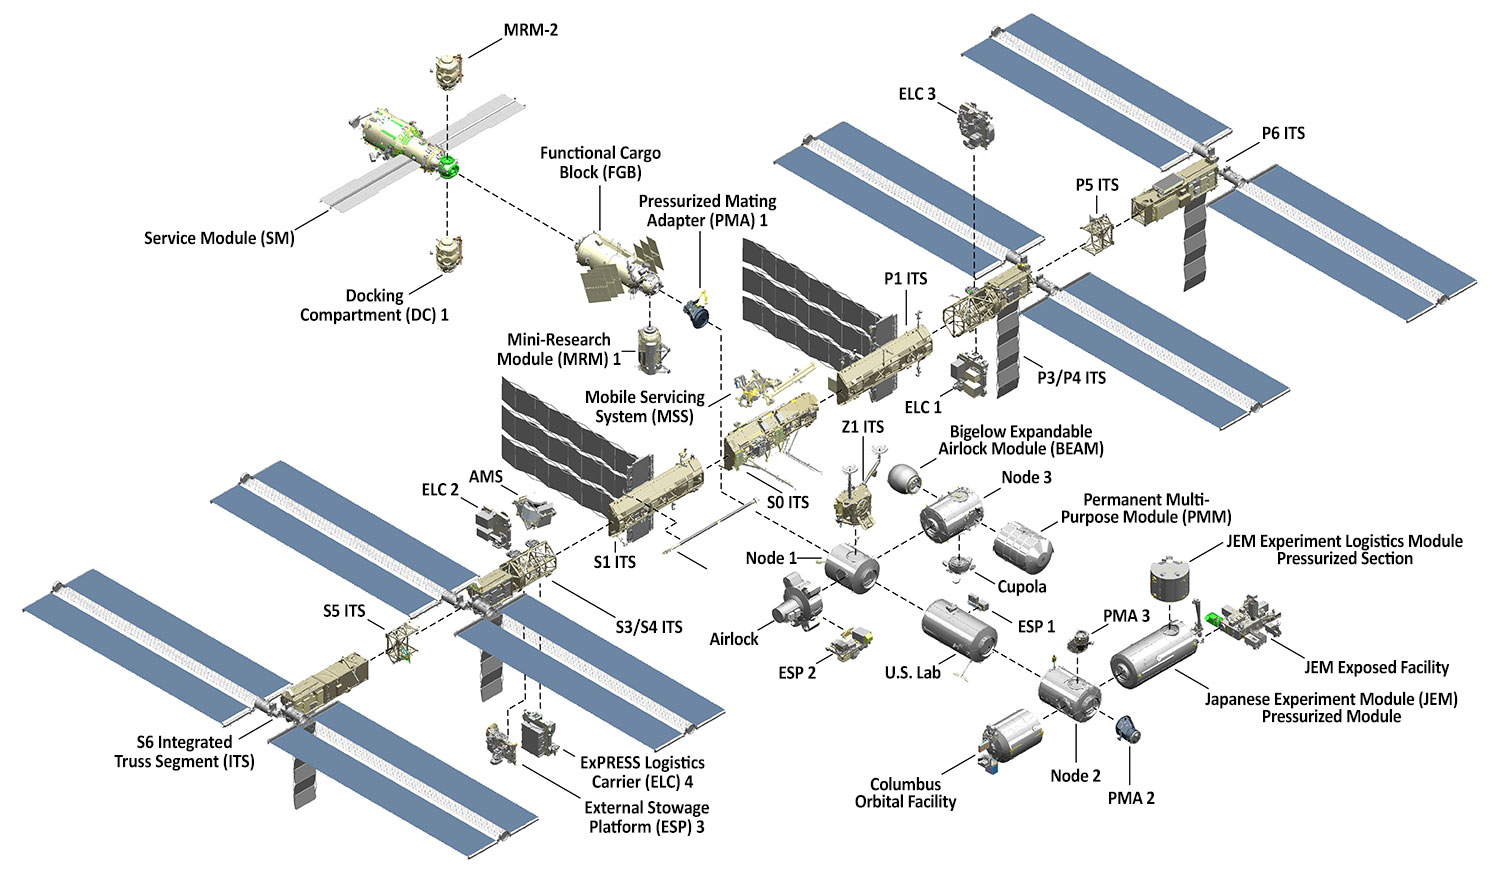
\includegraphics[width=\textwidth]{ISS_celek.jpg}
  \caption{Struktura Mezinárodní kosmické stanice \cite{ISS_facts}. Modul Columbus je dole uprostřed.}
  \label{fig:ISS_celek}
\end{figure}

Na obr. \ref{fig:ISS_celek} je vidět struktura stanice. Páteří stanice je 109~m dlouhý nosník~\cite{ISS_facts}, tzv. Integrated Truss Structure, ke kterému jsou připojeny fotovoltaické panely, moduly ISS a další části. Stanice byla postavena postupným skládáním přímo na orbitě, což si vyžádalo desítky kosmických letů. Zatím poslední připojená část BEAM (Bigelow Expandable Activity Module, nafukovací modul) byla vynesena na orbitu v roce 2016~\cite{ISS_gifs}. V tab. \ref{tab:ISS_parametry} jsou k dispozici základní parametry stanice.
\begin{table}[h]
  \centering
  \caption{Základní parametry ISS~\cite{ISS_facts}.}
  \label{tab:ISS_parametry}
  \begin{tabular}{ll}
    \toprule
    Délka obyvatelné části (s atmosférou)&73 m\\
    Délka hlavního nosníku&109 m\\
    Délka solárních panelů&73 m\\
    Hmotnost&419 725 kg\\
    Obytný objem& 388 m$^3$ (bez zahrnutí navštěvujících vozidel)\\
    Objem pod tlakem&916 m$^3$ (s BEAM modulem 932 m$^3$)\\
    % With BEAM expanded: 32,898 cubic feet (932 cubic meters)
    Zdroj energie& 8 solárních panelů (84 kW)\\
    %Počet řádků počítačového kódu& přibližně 2 300 000 \\
    \bottomrule
  \end{tabular}
\end{table}

Stanice je rozdělena na ruskou a americkou část. Zatímco ruská podléhá výhradně Rusům, americká se skládá z modulů a konstrukcí evropských, japonských, kanadských a amerických. ESA (European Space Agency, Evropská kosmická agentura) je zodpovědná za modul Columbus a za ATV (Automated Transfer Vehicles, automatické transportní vozidla)~\cite{ISS_about}; podle dohod s NASA má ESA nárok na 51\% využití zdrojů modulu Columbus~\cite{ISS_wiki}.

ISS bude provozována minimálně do roku 2024~\cite{ISS_prodlouzeni} a celkové náklady na vybudování, provoz stanice do tohoto roku, výzkum atd. jsou odhadovány na 100 miliard eur, z nich cca 8 miliard je či bude hrazena ESA, resp. jejími 10 členskými zeměmi podílející se na programu (Belgie, Dánsko, Francie, Neměcko, Itálie, Nizozemí, Norsko, Španělsko, Švédsko and Švýcarsko)~\cite{ISS_cost}.
\section{Modul Columbus}\label{sec:ISS_columbus}
Modul Columbus je největším příspěvkem ESA k ISS.

Jedná se o laboratorní modul zaměřený na výzkum v biologii, materiálových vědách, fyziku tekutin a další výzkumy v mikrogravitaci. Obsahuje deset skříňových modulů pro experimenty (International Standard Payload Racks), každý z nich poskytuje nezávislé ovládání energie, chlazení a také komunikaci s pozemními dispečery a vědci. Navíc na vnější straně laboratoře jsou čtyři plošiny, na které jdou umístit vědecké přístroje. Modul je 7 m dlouhý, jeho průměr činí 4,5 m a váží 10 300 kg (vše jsou přibližné hodnoty)~\cite{columbus}.

Právě v tomto modulu probíhal experiment DOSIS a v současnosti běží experiment DOSIS3D. 
\begin{figure}[H]
  \centering
  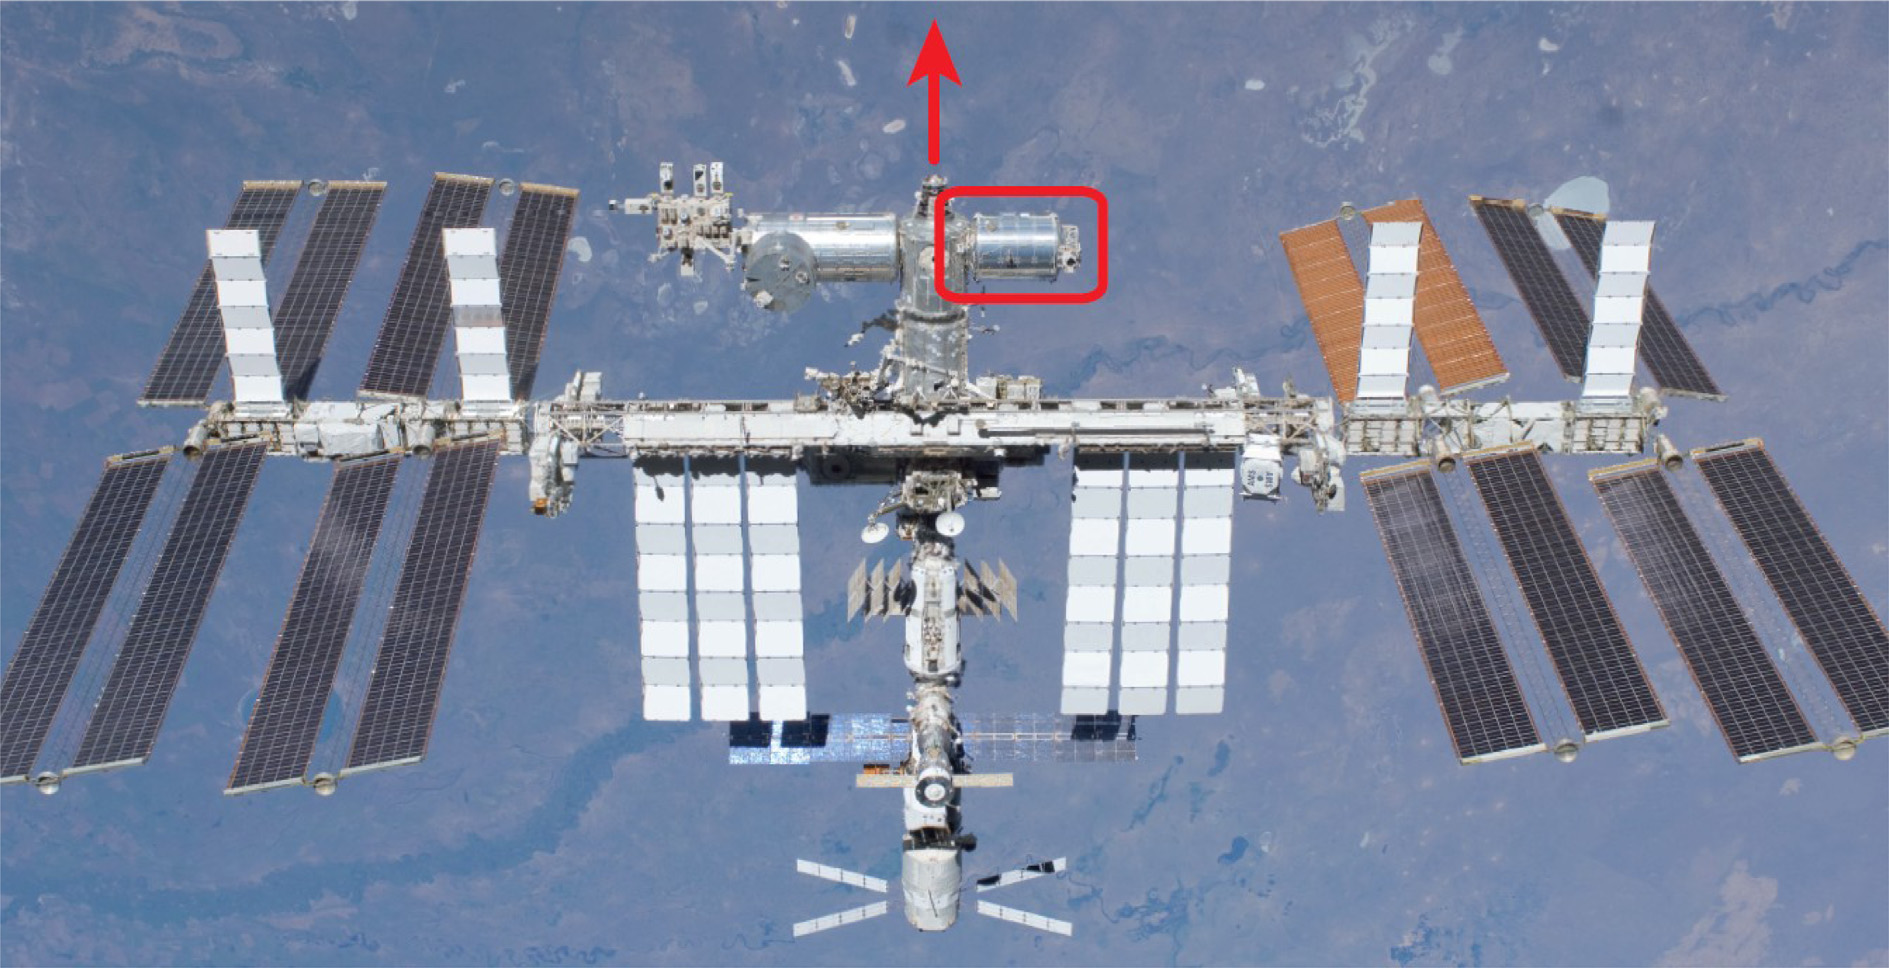
\includegraphics[width=0.8\textwidth]{ISS_columbus.png}
  \caption{Poloha modulu Columbus v rámci ISS je vyznačena červeně; červená šipka zobrazuje směr letu ISS~\cite{dosis}.}
  \label{fig:columbus_poloha}
\end{figure}
\begin{figure}[H]
  \centering
  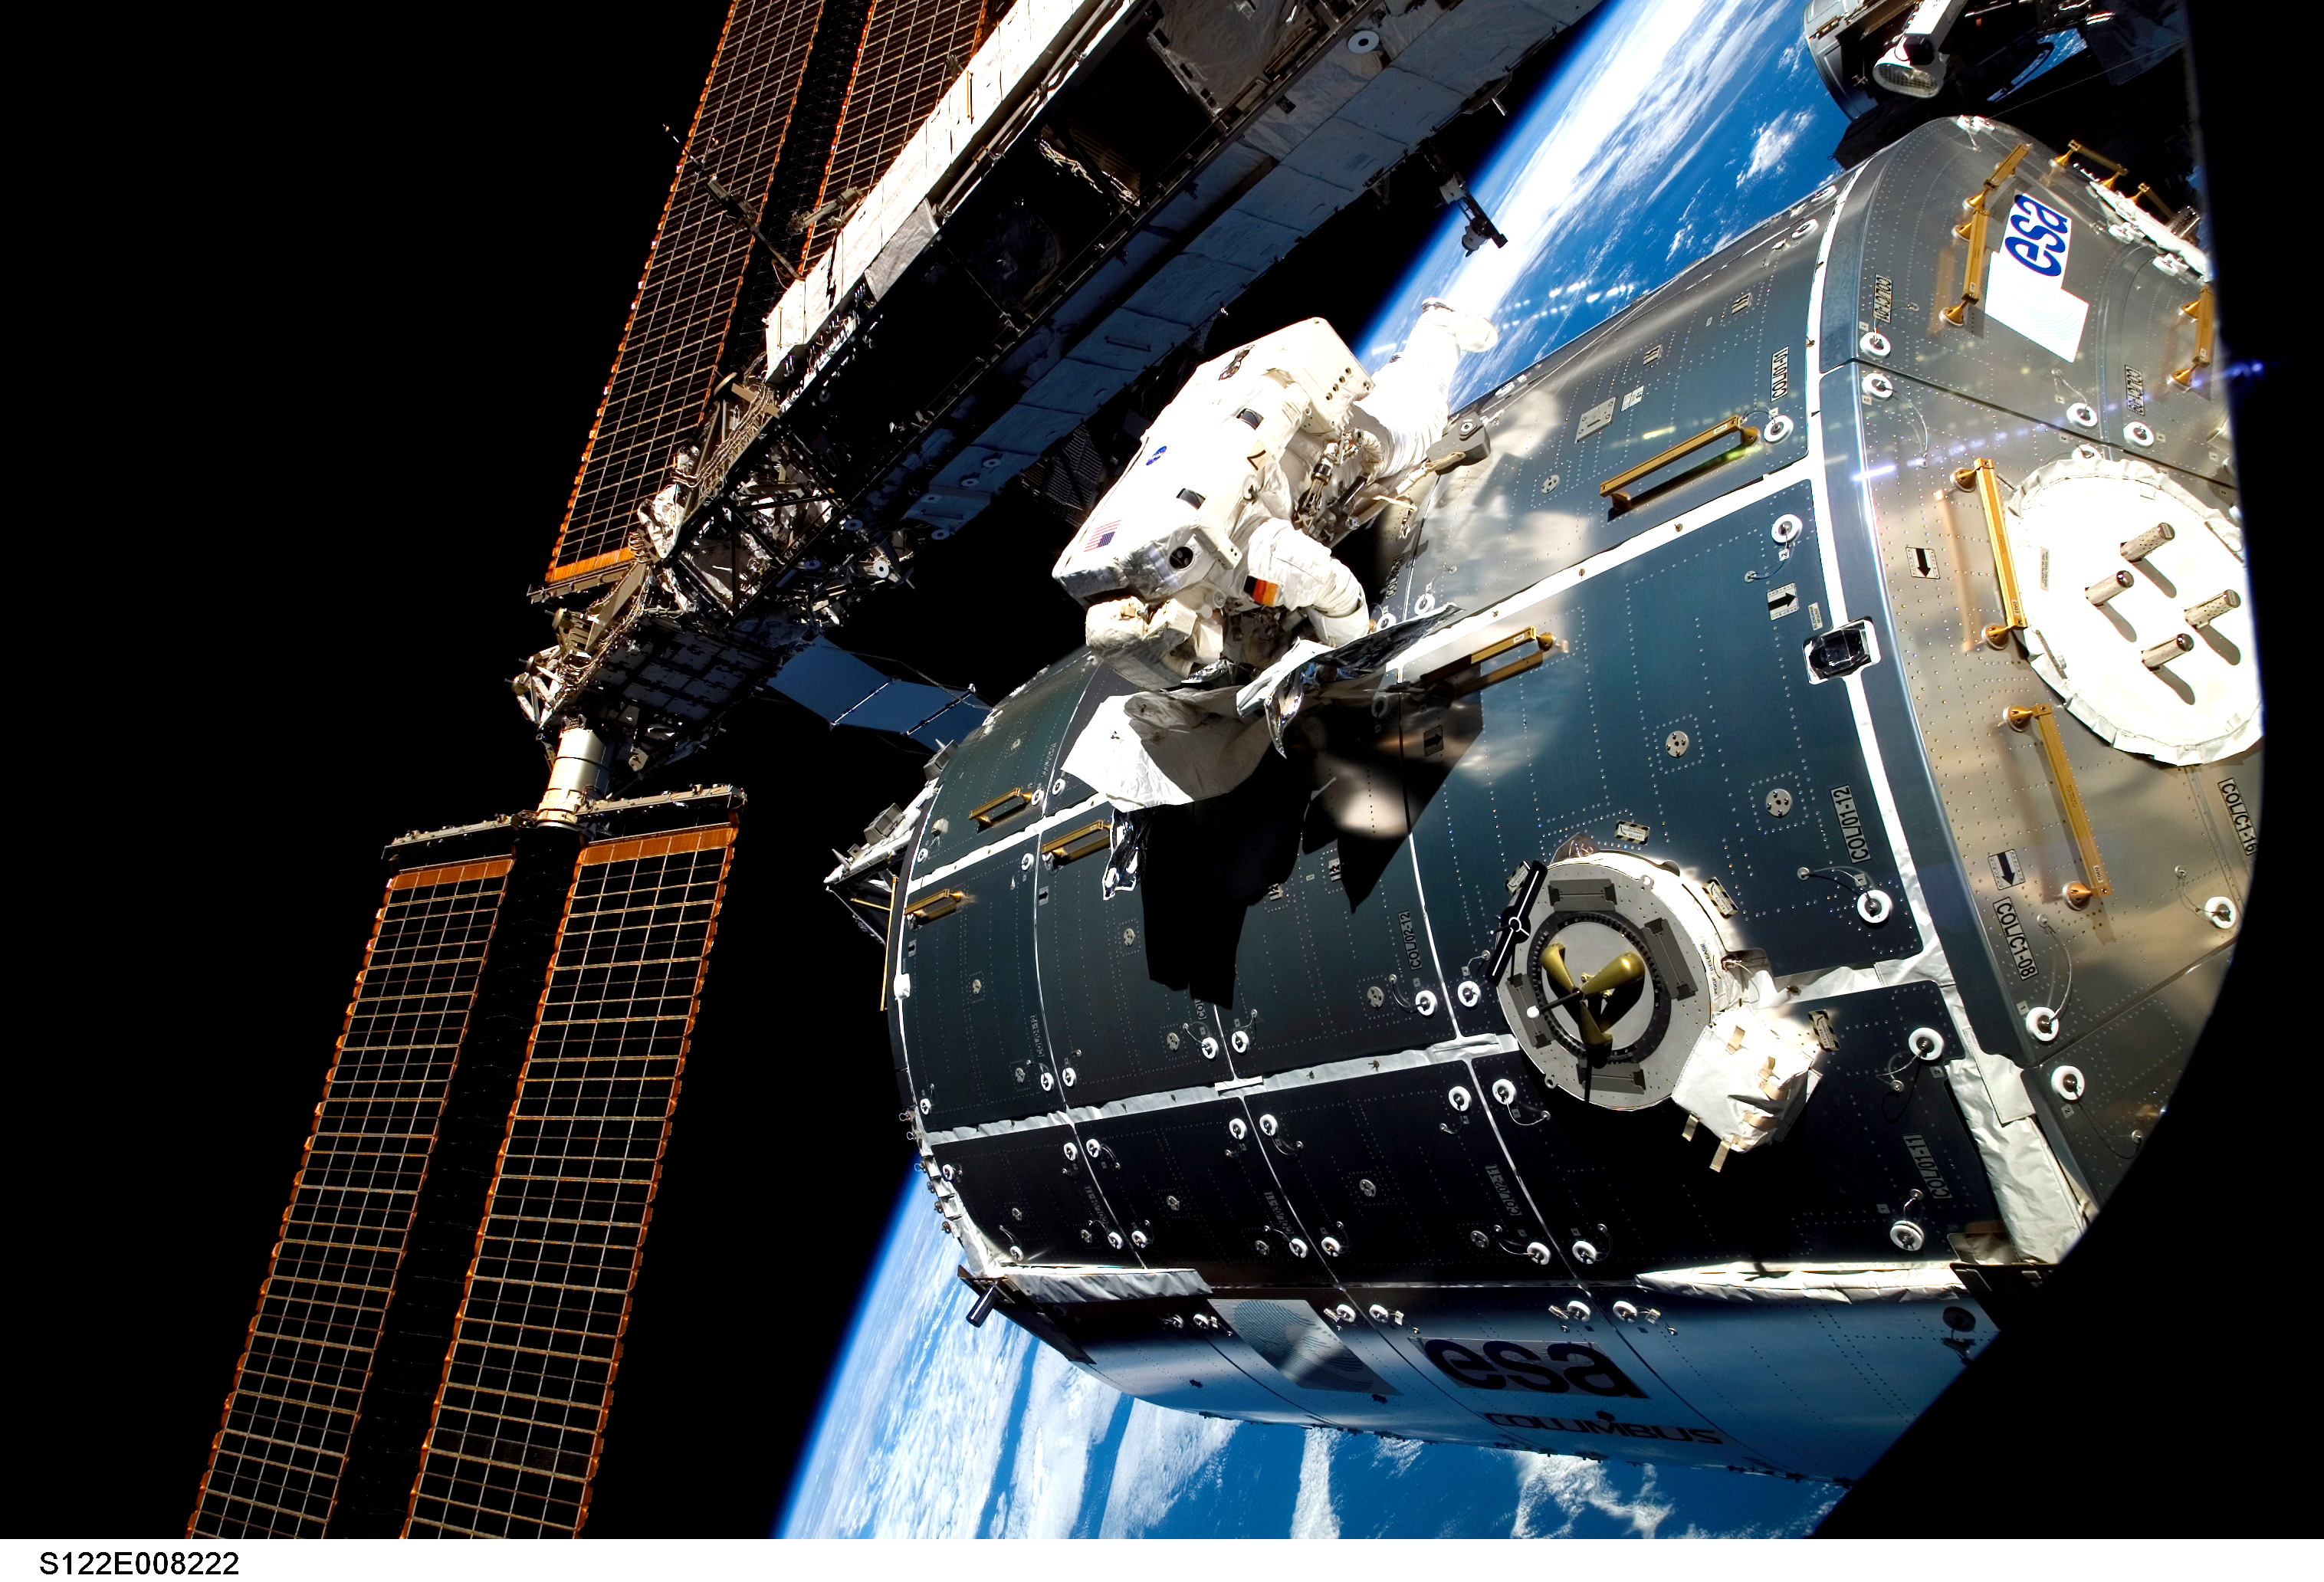
\includegraphics[width=0.8\textwidth]{columbus_outside.jpg}
  \caption{Modul Columbus ve srovnání s astronautem~\cite{columbus_outside}.}
  \label{fig:columbus_srovnani}
\end{figure}
%Informace obsažené v tomto oddíle byly brány z~\cite{columbus}.

